\documentclass[1p]{elsarticle_modified}
%\bibliographystyle{elsarticle-num}

%\usepackage[colorlinks]{hyperref}
%\usepackage{abbrmath_seonhwa} %\Abb, \Ascr, \Acal ,\Abf, \Afrak
\usepackage{amsfonts}
\usepackage{amssymb}
\usepackage{amsmath}
\usepackage{amsthm}
\usepackage{scalefnt}
\usepackage{amsbsy}
\usepackage{kotex}
\usepackage{caption}
\usepackage{subfig}
\usepackage{color}
\usepackage{graphicx}
\usepackage{xcolor} %% white, black, red, green, blue, cyan, magenta, yellow
\usepackage{float}
\usepackage{setspace}
\usepackage{hyperref}

\usepackage{tikz}
\usetikzlibrary{arrows}

\usepackage{multirow}
\usepackage{array} % fixed length table
\usepackage{hhline}

%%%%%%%%%%%%%%%%%%%%%
\makeatletter
\renewcommand*\env@matrix[1][\arraystretch]{%
	\edef\arraystretch{#1}%
	\hskip -\arraycolsep
	\let\@ifnextchar\new@ifnextchar
	\array{*\c@MaxMatrixCols c}}
\makeatother %https://tex.stackexchange.com/questions/14071/how-can-i-increase-the-line-spacing-in-a-matrix
%%%%%%%%%%%%%%%

\usepackage[normalem]{ulem}

\newcommand{\msout}[1]{\ifmmode\text{\sout{\ensuremath{#1}}}\else\sout{#1}\fi}
%SOURCE: \msout is \stkout macro in https://tex.stackexchange.com/questions/20609/strikeout-in-math-mode

\newcommand{\cancel}[1]{
	\ifmmode
	{\color{red}\msout{#1}}
	\else
	{\color{red}\sout{#1}}
	\fi
}

\newcommand{\add}[1]{
	{\color{blue}\uwave{#1}}
}

\newcommand{\replace}[2]{
	\ifmmode
	{\color{red}\msout{#1}}{\color{blue}\uwave{#2}}
	\else
	{\color{red}\sout{#1}}{\color{blue}\uwave{#2}}
	\fi
}

\newcommand{\Sol}{\mathcal{S}} %segment
\newcommand{\D}{D} %diagram
\newcommand{\A}{\mathcal{A}} %arc


%%%%%%%%%%%%%%%%%%%%%%%%%%%%%5 test

\def\sl{\operatorname{\textup{SL}}(2,\Cbb)}
\def\psl{\operatorname{\textup{PSL}}(2,\Cbb)}
\def\quan{\mkern 1mu \triangleright \mkern 1mu}

\theoremstyle{definition}
\newtheorem{thm}{Theorem}[section]
\newtheorem{prop}[thm]{Proposition}
\newtheorem{lem}[thm]{Lemma}
\newtheorem{ques}[thm]{Question}
\newtheorem{cor}[thm]{Corollary}
\newtheorem{defn}[thm]{Definition}
\newtheorem{exam}[thm]{Example}
\newtheorem{rmk}[thm]{Remark}
\newtheorem{alg}[thm]{Algorithm}

\newcommand{\I}{\sqrt{-1}}
\begin{document}

%\begin{frontmatter}
%
%\title{Boundary parabolic representations of knots up to 8 crossings}
%
%%% Group authors per affiliation:
%\author{Yunhi Cho} 
%\address{Department of Mathematics, University of Seoul, Seoul, Korea}
%\ead{yhcho@uos.ac.kr}
%
%
%\author{Seonhwa Kim} %\fnref{s_kim}}
%\address{Center for Geometry and Physics, Institute for Basic Science, Pohang, 37673, Korea}
%\ead{ryeona17@ibs.re.kr}
%
%\author{Hyuk Kim}
%\address{Department of Mathematical Sciences, Seoul National University, Seoul 08826, Korea}
%\ead{hyukkim@snu.ac.kr}
%
%\author{Seokbeom Yoon}
%\address{Department of Mathematical Sciences, Seoul National University, Seoul, 08826,  Korea}
%\ead{sbyoon15@snu.ac.kr}
%
%\begin{abstract}
%We find all boundary parabolic representation of knots up to 8 crossings.
%
%\end{abstract}
%\begin{keyword}
%    \MSC[2010] 57M25 
%\end{keyword}
%
%\end{frontmatter}

%\linenumbers
%\tableofcontents
%
\newcommand\colored[1]{\textcolor{white}{\rule[-0.35ex]{0.8em}{1.4ex}}\kern-0.8em\color{red} #1}%
%\newcommand\colored[1]{\textcolor{white}{ #1}\kern-2.17ex	\textcolor{white}{ #1}\kern-1.81ex	\textcolor{white}{ #1}\kern-2.15ex\color{red}#1	}

{\Large $\underline{12a_{0614}~(K12a_{0614})}$}

\setlength{\tabcolsep}{10pt}
\renewcommand{\arraystretch}{1.6}
\vspace{1cm}\begin{tabular}{m{100pt}>{\centering\arraybackslash}m{274pt}}
\multirow{5}{120pt}{
	\centering
	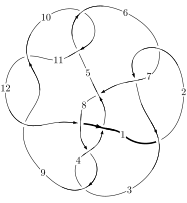
\includegraphics[width=112pt]{../../../GIT/diagram.site/Diagrams/png/1415_12a_0614.png}\\
\ \ \ A knot diagram\footnotemark}&
\allowdisplaybreaks
\textbf{Linearized knot diagam} \\
\cline{2-2}
 &
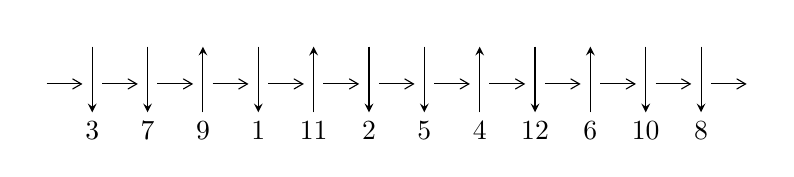
\begin{tikzpicture}[x=20pt, y=17pt]
	% nodes
	\node (C0) at (0, 0) {};
	\node (C1) at (1, 0) {};
	\node (C1U) at (1, +1) {};
	\node (C1D) at (1, -1) {3};

	\node (C2) at (2, 0) {};
	\node (C2U) at (2, +1) {};
	\node (C2D) at (2, -1) {7};

	\node (C3) at (3, 0) {};
	\node (C3U) at (3, +1) {};
	\node (C3D) at (3, -1) {9};

	\node (C4) at (4, 0) {};
	\node (C4U) at (4, +1) {};
	\node (C4D) at (4, -1) {1};

	\node (C5) at (5, 0) {};
	\node (C5U) at (5, +1) {};
	\node (C5D) at (5, -1) {11};

	\node (C6) at (6, 0) {};
	\node (C6U) at (6, +1) {};
	\node (C6D) at (6, -1) {2};

	\node (C7) at (7, 0) {};
	\node (C7U) at (7, +1) {};
	\node (C7D) at (7, -1) {5};

	\node (C8) at (8, 0) {};
	\node (C8U) at (8, +1) {};
	\node (C8D) at (8, -1) {4};

	\node (C9) at (9, 0) {};
	\node (C9U) at (9, +1) {};
	\node (C9D) at (9, -1) {12};

	\node (C10) at (10, 0) {};
	\node (C10U) at (10, +1) {};
	\node (C10D) at (10, -1) {6};

	\node (C11) at (11, 0) {};
	\node (C11U) at (11, +1) {};
	\node (C11D) at (11, -1) {10};

	\node (C12) at (12, 0) {};
	\node (C12U) at (12, +1) {};
	\node (C12D) at (12, -1) {8};
	\node (C13) at (13, 0) {};

	% arrows
	\draw[->,>={angle 60}]
	(C0) edge (C1) (C1) edge (C2) (C2) edge (C3) (C3) edge (C4) (C4) edge (C5) (C5) edge (C6) (C6) edge (C7) (C7) edge (C8) (C8) edge (C9) (C9) edge (C10) (C10) edge (C11) (C11) edge (C12) (C12) edge (C13) ;	\draw[->,>=stealth]
	(C1U) edge (C1D) (C2U) edge (C2D) (C3D) edge (C3U) (C4U) edge (C4D) (C5D) edge (C5U) (C6U) edge (C6D) (C7U) edge (C7D) (C8D) edge (C8U) (C9U) edge (C9D) (C10D) edge (C10U) (C11U) edge (C11D) (C12U) edge (C12D) ;
	\end{tikzpicture} \\
\hhline{~~} \\& 
\textbf{Solving Sequence} \\ \cline{2-2} 
 &
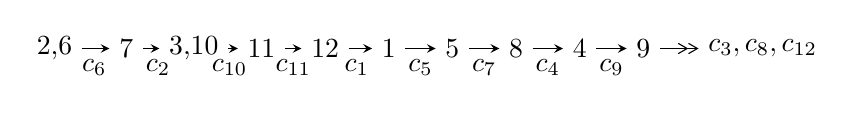
\begin{tikzpicture}[x=23pt, y=7pt]
	% node
	\node (A0) at (-1/8, 0) {2,6};
	\node (A1) at (1, 0) {7};
	\node (A2) at (33/16, 0) {3,10};
	\node (A3) at (25/8, 0) {11};
	\node (A4) at (33/8, 0) {12};
	\node (A5) at (41/8, 0) {1};
	\node (A6) at (49/8, 0) {5};
	\node (A7) at (57/8, 0) {8};
	\node (A8) at (65/8, 0) {4};
	\node (A9) at (73/8, 0) {9};
	\node (C1) at (1/2, -1) {$c_{6}$};
	\node (C2) at (3/2, -1) {$c_{2}$};
	\node (C3) at (21/8, -1) {$c_{10}$};
	\node (C4) at (29/8, -1) {$c_{11}$};
	\node (C5) at (37/8, -1) {$c_{1}$};
	\node (C6) at (45/8, -1) {$c_{5}$};
	\node (C7) at (53/8, -1) {$c_{7}$};
	\node (C8) at (61/8, -1) {$c_{4}$};
	\node (C9) at (69/8, -1) {$c_{9}$};
	\node (A10) at (11, 0) {$c_{3},c_{8},c_{12}$};

	% edge
	\draw[->,>=stealth]	
	(A0) edge (A1) (A1) edge (A2) (A2) edge (A3) (A3) edge (A4) (A4) edge (A5) (A5) edge (A6) (A6) edge (A7) (A7) edge (A8) (A8) edge (A9) ;
	\draw[->>,>={angle 60}]	
	(A9) edge (A10);
\end{tikzpicture} \\ 

\end{tabular} \\

\footnotetext{
The image of knot diagram is generated by the software ``\textbf{Draw programme}" developed by Andrew Bartholomew(\url{http://www.layer8.co.uk/maths/draw/index.htm\#Running-draw}), where we modified some parts for our purpose(\url{https://github.com/CATsTAILs/LinksPainter}).
}\phantom \\ \newline 
\centering \textbf{Ideals for irreducible components\footnotemark of $X_{\text{par}}$} 
 
\begin{align*}
I^u_{1}&=\langle 
3.92933\times10^{370} u^{134}-5.89479\times10^{371} u^{133}+\cdots+7.41919\times10^{372} b+1.34218\times10^{374},\\
\phantom{I^u_{1}}&\phantom{= \langle  }-1.76780\times10^{374} u^{134}+9.66876\times10^{373} u^{133}+\cdots+1.23900\times10^{375} a+4.89956\times10^{376},\\
\phantom{I^u_{1}}&\phantom{= \langle  }u^{135}- u^{134}+\cdots+885 u+167\rangle \\
I^u_{2}&=\langle 
7 u^{27}-42 u^{25}+\cdots+16 u^3+b,\;18 u^{27}+3 u^{26}+\cdots+a+18,\;u^{28}-7 u^{26}+\cdots+u+1\rangle \\
\\
\end{align*}
\raggedright * 2 irreducible components of $\dim_{\mathbb{C}}=0$, with total 163 representations.\\
\footnotetext{All coefficients of polynomials are rational numbers. But the coefficients are sometimes approximated in decimal forms when there is not enough margin.}
\newpage
\renewcommand{\arraystretch}{1}
\centering \section*{I. $I^u_{1}= \langle 3.93\times10^{370} u^{134}-5.89\times10^{371} u^{133}+\cdots+7.42\times10^{372} b+1.34\times10^{374},\;-1.77\times10^{374} u^{134}+9.67\times10^{373} u^{133}+\cdots+1.24\times10^{375} a+4.90\times10^{376},\;u^{135}- u^{134}+\cdots+885 u+167 \rangle$}
\flushleft \textbf{(i) Arc colorings}\\
\begin{tabular}{m{7pt} m{180pt} m{7pt} m{180pt} }
\flushright $a_{2}=$&$\begin{pmatrix}0\\u\end{pmatrix}$ \\
\flushright $a_{6}=$&$\begin{pmatrix}1\\0\end{pmatrix}$ \\
\flushright $a_{7}=$&$\begin{pmatrix}1\\u^2\end{pmatrix}$ \\
\flushright $a_{3}=$&$\begin{pmatrix}- u\\- u^3+u\end{pmatrix}$ \\
\flushright $a_{10}=$&$\begin{pmatrix}0.142679 u^{134}-0.0780365 u^{133}+\cdots-229.717 u-39.5443\\-0.00529617 u^{134}+0.0794533 u^{133}+\cdots-109.718 u-18.0906\end{pmatrix}$ \\
\flushright $a_{11}=$&$\begin{pmatrix}0.137383 u^{134}+0.00141679 u^{133}+\cdots-339.435 u-57.6350\\-0.00529617 u^{134}+0.0794533 u^{133}+\cdots-109.718 u-18.0906\end{pmatrix}$ \\
\flushright $a_{12}=$&$\begin{pmatrix}0.194027 u^{134}-0.207818 u^{133}+\cdots-154.835 u-20.4301\\0.0171057 u^{134}+0.137564 u^{133}+\cdots-258.968 u-42.2172\end{pmatrix}$ \\
\flushright $a_{1}=$&$\begin{pmatrix}u^3\\u^5- u^3+u\end{pmatrix}$ \\
\flushright $a_{5}=$&$\begin{pmatrix}0.0205101 u^{134}+0.0101705 u^{133}+\cdots+111.884 u+22.4781\\0.0705745 u^{134}-0.0503292 u^{133}+\cdots+34.2145 u+5.86546\end{pmatrix}$ \\
\flushright $a_{8}=$&$\begin{pmatrix}0.182694 u^{134}-0.204743 u^{133}+\cdots-91.6431 u-11.8583\\0.0395044 u^{134}+0.0248050 u^{133}+\cdots-154.329 u-23.1275\end{pmatrix}$ \\
\flushright $a_{4}=$&$\begin{pmatrix}-0.0347015 u^{134}+0.0132842 u^{133}+\cdots+141.961 u+26.9193\\0.0488055 u^{134}-0.0622889 u^{133}+\cdots+41.3893 u+6.84940\end{pmatrix}$ \\
\flushright $a_{9}=$&$\begin{pmatrix}0.0665998 u^{134}-0.110583 u^{133}+\cdots+4.15920 u-3.32764\\-0.0825305 u^{134}+0.0961945 u^{133}+\cdots+31.4168 u+5.45217\end{pmatrix}$\\&\end{tabular}
\flushleft \textbf{(ii) Obstruction class $= -1$}\\~\\
\flushleft \textbf{(iii) Cusp Shapes $= 0.591980 u^{134}-0.176380 u^{133}+\cdots-933.156 u-154.184$}\\~\\
\newpage\renewcommand{\arraystretch}{1}
\flushleft \textbf{(iv) u-Polynomials at the component}\newline \\
\begin{tabular}{m{50pt}|m{274pt}}
Crossings & \hspace{64pt}u-Polynomials at each crossing \\
\hline $$\begin{aligned}c_{1}\end{aligned}$$&$\begin{aligned}
&u^{135}+55 u^{134}+\cdots+544081 u+27889
\end{aligned}$\\
\hline $$\begin{aligned}c_{2},c_{6}\end{aligned}$$&$\begin{aligned}
&u^{135}- u^{134}+\cdots+885 u+167
\end{aligned}$\\
\hline $$\begin{aligned}c_{3},c_{8}\end{aligned}$$&$\begin{aligned}
&u^{135}- u^{134}+\cdots+8241 u+1341
\end{aligned}$\\
\hline $$\begin{aligned}c_{4}\end{aligned}$$&$\begin{aligned}
&u^{135}-3 u^{134}+\cdots-54 u+1
\end{aligned}$\\
\hline $$\begin{aligned}c_{5},c_{10}\end{aligned}$$&$\begin{aligned}
&u^{135}+u^{134}+\cdots+315 u+43
\end{aligned}$\\
\hline $$\begin{aligned}c_{7}\end{aligned}$$&$\begin{aligned}
&u^{135}-4 u^{134}+\cdots-3344250 u+838321
\end{aligned}$\\
\hline $$\begin{aligned}c_{9},c_{11}\end{aligned}$$&$\begin{aligned}
&u^{135}+43 u^{134}+\cdots-46545 u-1849
\end{aligned}$\\
\hline $$\begin{aligned}c_{12}\end{aligned}$$&$\begin{aligned}
&u^{135}-3 u^{134}+\cdots+44 u-1
\end{aligned}$\\
\hline
\end{tabular}\\~\\
\newpage\renewcommand{\arraystretch}{1}
\flushleft \textbf{(v) Riley Polynomials at the component}\newline \\
\begin{tabular}{m{50pt}|m{274pt}}
Crossings & \hspace{64pt}Riley Polynomials at each crossing \\
\hline $$\begin{aligned}c_{1}\end{aligned}$$&$\begin{aligned}
&y^{135}+65 y^{134}+\cdots-226517556159 y-777796321
\end{aligned}$\\
\hline $$\begin{aligned}c_{2},c_{6}\end{aligned}$$&$\begin{aligned}
&y^{135}-55 y^{134}+\cdots+544081 y-27889
\end{aligned}$\\
\hline $$\begin{aligned}c_{3},c_{8}\end{aligned}$$&$\begin{aligned}
&y^{135}+79 y^{134}+\cdots-103538133 y-1798281
\end{aligned}$\\
\hline $$\begin{aligned}c_{4}\end{aligned}$$&$\begin{aligned}
&y^{135}-11 y^{134}+\cdots+230 y-1
\end{aligned}$\\
\hline $$\begin{aligned}c_{5},c_{10}\end{aligned}$$&$\begin{aligned}
&y^{135}+43 y^{134}+\cdots-46545 y-1849
\end{aligned}$\\
\hline $$\begin{aligned}c_{7}\end{aligned}$$&$\begin{aligned}
&y^{135}+30 y^{134}+\cdots-25519271420832 y-702782099041
\end{aligned}$\\
\hline $$\begin{aligned}c_{9},c_{11}\end{aligned}$$&$\begin{aligned}
&y^{135}+111 y^{134}+\cdots+44824163 y-3418801
\end{aligned}$\\
\hline $$\begin{aligned}c_{12}\end{aligned}$$&$\begin{aligned}
&y^{135}-5 y^{134}+\cdots-346 y-1
\end{aligned}$\\
\hline
\end{tabular}\\~\\
\newpage\flushleft \textbf{(vi) Complex Volumes and Cusp Shapes}
$$\begin{array}{c|c|c}  
\text{Solutions to }I^u_{1}& \I (\text{vol} + \sqrt{-1}CS) & \text{Cusp shape}\\
 \hline 
\begin{aligned}
u &= \phantom{-}0.837846 + 0.549307 I \\
a &= \phantom{-}3.47986 + 0.41455 I \\
b &= -0.727872 + 0.868167 I\end{aligned}
 & \phantom{-}0.488345 - 1.251270 I & \phantom{-0.000000 } 0 \\ \hline\begin{aligned}
u &= \phantom{-}0.837846 - 0.549307 I \\
a &= \phantom{-}3.47986 - 0.41455 I \\
b &= -0.727872 - 0.868167 I\end{aligned}
 & \phantom{-}0.488345 + 1.251270 I & \phantom{-0.000000 } 0 \\ \hline\begin{aligned}
u &= \phantom{-}0.738899 + 0.681368 I \\
a &= -0.945762 - 0.131379 I \\
b &= \phantom{-}0.645324 - 0.176703 I\end{aligned}
 & \phantom{-}2.85702 - 0.94017 I & \phantom{-0.000000 } 0 \\ \hline\begin{aligned}
u &= \phantom{-}0.738899 - 0.681368 I \\
a &= -0.945762 + 0.131379 I \\
b &= \phantom{-}0.645324 + 0.176703 I\end{aligned}
 & \phantom{-}2.85702 + 0.94017 I & \phantom{-0.000000 } 0 \\ \hline\begin{aligned}
u &= -0.801992 + 0.582367 I \\
a &= \phantom{-}1.77385 + 0.10818 I \\
b &= -0.946357 - 0.853076 I\end{aligned}
 & \phantom{-}5.44949 + 4.76272 I & \phantom{-0.000000 } 0 \\ \hline\begin{aligned}
u &= -0.801992 - 0.582367 I \\
a &= \phantom{-}1.77385 - 0.10818 I \\
b &= -0.946357 + 0.853076 I\end{aligned}
 & \phantom{-}5.44949 - 4.76272 I & \phantom{-0.000000 } 0 \\ \hline\begin{aligned}
u &= \phantom{-}0.569934 + 0.836668 I \\
a &= \phantom{-}1.45649 - 0.70116 I \\
b &= -0.848678 + 0.794378 I\end{aligned}
 & \phantom{-}7.77386 + 0.60727 I & \phantom{-0.000000 } 0 \\ \hline\begin{aligned}
u &= \phantom{-}0.569934 - 0.836668 I \\
a &= \phantom{-}1.45649 + 0.70116 I \\
b &= -0.848678 - 0.794378 I\end{aligned}
 & \phantom{-}7.77386 - 0.60727 I & \phantom{-0.000000 } 0 \\ \hline\begin{aligned}
u &= -0.521046 + 0.834885 I \\
a &= \phantom{-}1.66324 - 0.38714 I \\
b &= -0.784742 + 0.975593 I\end{aligned}
 & \phantom{-}7.21061 - 6.69518 I & \phantom{-0.000000 } 0 \\ \hline\begin{aligned}
u &= -0.521046 - 0.834885 I \\
a &= \phantom{-}1.66324 + 0.38714 I \\
b &= -0.784742 - 0.975593 I\end{aligned}
 & \phantom{-}7.21061 + 6.69518 I & \phantom{-0.000000 } 0\\
 \hline 
 \end{array}$$\newpage$$\begin{array}{c|c|c}  
\text{Solutions to }I^u_{1}& \I (\text{vol} + \sqrt{-1}CS) & \text{Cusp shape}\\
 \hline 
\begin{aligned}
u &= \phantom{-}1.015020 + 0.089474 I \\
a &= -0.443199 - 0.837408 I \\
b &= \phantom{-}0.690637 + 0.366255 I\end{aligned}
 & -4.17899 + 2.70950 I & \phantom{-0.000000 } 0 \\ \hline\begin{aligned}
u &= \phantom{-}1.015020 - 0.089474 I \\
a &= -0.443199 + 0.837408 I \\
b &= \phantom{-}0.690637 - 0.366255 I\end{aligned}
 & -4.17899 - 2.70950 I & \phantom{-0.000000 } 0 \\ \hline\begin{aligned}
u &= -0.772593 + 0.591990 I \\
a &= \phantom{-}0.98832 - 2.34518 I \\
b &= -0.725888 + 0.881649 I\end{aligned}
 & \phantom{-}0.44638 - 4.29353 I & \phantom{-0.000000 } 0 \\ \hline\begin{aligned}
u &= -0.772593 - 0.591990 I \\
a &= \phantom{-}0.98832 + 2.34518 I \\
b &= -0.725888 - 0.881649 I\end{aligned}
 & \phantom{-}0.44638 + 4.29353 I & \phantom{-0.000000 } 0 \\ \hline\begin{aligned}
u &= \phantom{-}0.879122 + 0.553894 I \\
a &= -1.47816 - 1.86865 I \\
b &= \phantom{-}0.785743 + 0.814817 I\end{aligned}
 & \phantom{-}0.34887 - 3.16762 I & \phantom{-0.000000 } 0 \\ \hline\begin{aligned}
u &= \phantom{-}0.879122 - 0.553894 I \\
a &= -1.47816 + 1.86865 I \\
b &= \phantom{-}0.785743 - 0.814817 I\end{aligned}
 & \phantom{-}0.34887 + 3.16762 I & \phantom{-0.000000 } 0 \\ \hline\begin{aligned}
u &= -0.247760 + 0.918909 I \\
a &= \phantom{-}1.74816 + 0.53629 I \\
b &= -0.823192 - 0.895739 I\end{aligned}
 & \phantom{-}6.21835 + 3.18298 I & \phantom{-0.000000 } 0 \\ \hline\begin{aligned}
u &= -0.247760 - 0.918909 I \\
a &= \phantom{-}1.74816 - 0.53629 I \\
b &= -0.823192 + 0.895739 I\end{aligned}
 & \phantom{-}6.21835 - 3.18298 I & \phantom{-0.000000 } 0 \\ \hline\begin{aligned}
u &= \phantom{-}0.986857 + 0.374682 I \\
a &= \phantom{-}0.11667 - 1.73761 I \\
b &= -0.052535 - 1.031140 I\end{aligned}
 & -6.17843 - 1.22320 I & \phantom{-0.000000 } 0 \\ \hline\begin{aligned}
u &= \phantom{-}0.986857 - 0.374682 I \\
a &= \phantom{-}0.11667 + 1.73761 I \\
b &= -0.052535 + 1.031140 I\end{aligned}
 & -6.17843 + 1.22320 I & \phantom{-0.000000 } 0\\
 \hline 
 \end{array}$$\newpage$$\begin{array}{c|c|c}  
\text{Solutions to }I^u_{1}& \I (\text{vol} + \sqrt{-1}CS) & \text{Cusp shape}\\
 \hline 
\begin{aligned}
u &= \phantom{-}0.198122 + 0.921347 I \\
a &= \phantom{-}1.58183 + 0.70299 I \\
b &= -0.819161 - 0.899719 I\end{aligned}
 & \phantom{-}6.20339 + 2.94822 I & \phantom{-0.000000 } 0 \\ \hline\begin{aligned}
u &= \phantom{-}0.198122 - 0.921347 I \\
a &= \phantom{-}1.58183 - 0.70299 I \\
b &= -0.819161 + 0.899719 I\end{aligned}
 & \phantom{-}6.20339 - 2.94822 I & \phantom{-0.000000 } 0 \\ \hline\begin{aligned}
u &= \phantom{-}0.900622 + 0.258632 I \\
a &= -1.69639 - 2.72780 I \\
b &= -0.058372 - 0.785928 I\end{aligned}
 & -3.18317 + 1.73612 I & \phantom{-0.000000 } 0 \\ \hline\begin{aligned}
u &= \phantom{-}0.900622 - 0.258632 I \\
a &= -1.69639 + 2.72780 I \\
b &= -0.058372 + 0.785928 I\end{aligned}
 & -3.18317 - 1.73612 I & \phantom{-0.000000 } 0 \\ \hline\begin{aligned}
u &= \phantom{-}0.923325 + 0.113739 I \\
a &= \phantom{-}1.10579 + 2.21213 I \\
b &= -0.320453 + 0.887390 I\end{aligned}
 & -3.72106 - 2.39646 I & \phantom{-0.000000 } 0 \\ \hline\begin{aligned}
u &= \phantom{-}0.923325 - 0.113739 I \\
a &= \phantom{-}1.10579 - 2.21213 I \\
b &= -0.320453 - 0.887390 I\end{aligned}
 & -3.72106 + 2.39646 I & \phantom{-0.000000 } 0 \\ \hline\begin{aligned}
u &= \phantom{-}1.028760 + 0.297636 I \\
a &= \phantom{-}1.45891 + 0.31108 I \\
b &= -0.211476 - 0.392322 I\end{aligned}
 & -3.81731 - 3.79382 I & \phantom{-0.000000 } 0 \\ \hline\begin{aligned}
u &= \phantom{-}1.028760 - 0.297636 I \\
a &= \phantom{-}1.45891 - 0.31108 I \\
b &= -0.211476 + 0.392322 I\end{aligned}
 & -3.81731 + 3.79382 I & \phantom{-0.000000 } 0 \\ \hline\begin{aligned}
u &= -0.856282 + 0.644920 I \\
a &= -0.935673 + 0.291087 I \\
b &= -0.028328 + 1.233560 I\end{aligned}
 & -1.77111 + 2.51661 I & \phantom{-0.000000 } 0 \\ \hline\begin{aligned}
u &= -0.856282 - 0.644920 I \\
a &= -0.935673 - 0.291087 I \\
b &= -0.028328 - 1.233560 I\end{aligned}
 & -1.77111 - 2.51661 I & \phantom{-0.000000 } 0\\
 \hline 
 \end{array}$$\newpage$$\begin{array}{c|c|c}  
\text{Solutions to }I^u_{1}& \I (\text{vol} + \sqrt{-1}CS) & \text{Cusp shape}\\
 \hline 
\begin{aligned}
u &= \phantom{-}0.761538 + 0.520822 I \\
a &= \phantom{-}1.065400 + 0.896290 I \\
b &= -0.884082 - 0.986812 I\end{aligned}
 & \phantom{-}5.03019 + 1.92758 I & \phantom{-0.000000 } 0 \\ \hline\begin{aligned}
u &= \phantom{-}0.761538 - 0.520822 I \\
a &= \phantom{-}1.065400 - 0.896290 I \\
b &= -0.884082 + 0.986812 I\end{aligned}
 & \phantom{-}5.03019 - 1.92758 I & \phantom{-0.000000 } 0 \\ \hline\begin{aligned}
u &= \phantom{-}0.861221 + 0.319500 I \\
a &= -0.89814 + 1.16750 I \\
b &= \phantom{-}0.675323 + 1.002060 I\end{aligned}
 & -1.70069 + 4.51817 I & \phantom{-0.000000 } 0 \\ \hline\begin{aligned}
u &= \phantom{-}0.861221 - 0.319500 I \\
a &= -0.89814 - 1.16750 I \\
b &= \phantom{-}0.675323 - 1.002060 I\end{aligned}
 & -1.70069 - 4.51817 I & \phantom{-0.000000 } 0 \\ \hline\begin{aligned}
u &= -0.751154 + 0.780296 I \\
a &= -1.059250 + 0.743059 I \\
b &= \phantom{-}0.769638 - 1.038270 I\end{aligned}
 & \phantom{-}4.31054 - 4.50108 I & \phantom{-0.000000 } 0 \\ \hline\begin{aligned}
u &= -0.751154 - 0.780296 I \\
a &= -1.059250 - 0.743059 I \\
b &= \phantom{-}0.769638 + 1.038270 I\end{aligned}
 & \phantom{-}4.31054 + 4.50108 I & \phantom{-0.000000 } 0 \\ \hline\begin{aligned}
u &= -0.583906 + 0.704669 I \\
a &= \phantom{-}0.994060 - 0.654478 I \\
b &= -0.807640 - 0.029711 I\end{aligned}
 & \phantom{-}0.64232 - 3.58642 I & \phantom{-0.000000 } 0 \\ \hline\begin{aligned}
u &= -0.583906 - 0.704669 I \\
a &= \phantom{-}0.994060 + 0.654478 I \\
b &= -0.807640 + 0.029711 I\end{aligned}
 & \phantom{-}0.64232 + 3.58642 I & \phantom{-0.000000 } 0 \\ \hline\begin{aligned}
u &= -1.088150 + 0.046799 I \\
a &= \phantom{-}0.007861 - 0.437998 I \\
b &= \phantom{-}0.739339 - 0.837483 I\end{aligned}
 & \phantom{-}1.61109 - 0.51782 I & \phantom{-0.000000 } 0 \\ \hline\begin{aligned}
u &= -1.088150 - 0.046799 I \\
a &= \phantom{-}0.007861 + 0.437998 I \\
b &= \phantom{-}0.739339 + 0.837483 I\end{aligned}
 & \phantom{-}1.61109 + 0.51782 I & \phantom{-0.000000 } 0\\
 \hline 
 \end{array}$$\newpage$$\begin{array}{c|c|c}  
\text{Solutions to }I^u_{1}& \I (\text{vol} + \sqrt{-1}CS) & \text{Cusp shape}\\
 \hline 
\begin{aligned}
u &= \phantom{-}0.408397 + 0.813659 I \\
a &= \phantom{-}0.144674 + 0.121440 I \\
b &= -0.299766 - 1.080180 I\end{aligned}
 & -2.87341 + 7.30102 I & \phantom{-0.000000 } 0 \\ \hline\begin{aligned}
u &= \phantom{-}0.408397 - 0.813659 I \\
a &= \phantom{-}0.144674 - 0.121440 I \\
b &= -0.299766 + 1.080180 I\end{aligned}
 & -2.87341 - 7.30102 I & \phantom{-0.000000 } 0 \\ \hline\begin{aligned}
u &= -0.900828 + 0.617380 I \\
a &= -0.259939 + 1.214590 I \\
b &= \phantom{-}0.914727 - 0.770669 I\end{aligned}
 & \phantom{-}5.11294 - 0.01279 I & \phantom{-0.000000 } 0 \\ \hline\begin{aligned}
u &= -0.900828 - 0.617380 I \\
a &= -0.259939 - 1.214590 I \\
b &= \phantom{-}0.914727 + 0.770669 I\end{aligned}
 & \phantom{-}5.11294 + 0.01279 I & \phantom{-0.000000 } 0 \\ \hline\begin{aligned}
u &= -0.822721 + 0.380864 I \\
a &= -0.243214 + 0.016316 I \\
b &= \phantom{-}0.728615 + 0.639865 I\end{aligned}
 & -0.643269 + 0.860111 I & \phantom{-0.000000 } 0 \\ \hline\begin{aligned}
u &= -0.822721 - 0.380864 I \\
a &= -0.243214 - 0.016316 I \\
b &= \phantom{-}0.728615 - 0.639865 I\end{aligned}
 & -0.643269 - 0.860111 I & \phantom{-0.000000 } 0 \\ \hline\begin{aligned}
u &= -0.922603 + 0.587180 I \\
a &= -2.95088 - 0.29973 I \\
b &= \phantom{-}0.753223 + 0.938531 I\end{aligned}
 & -0.03377 + 8.97195 I & \phantom{-0.000000 } 0 \\ \hline\begin{aligned}
u &= -0.922603 - 0.587180 I \\
a &= -2.95088 + 0.29973 I \\
b &= \phantom{-}0.753223 - 0.938531 I\end{aligned}
 & -0.03377 - 8.97195 I & \phantom{-0.000000 } 0 \\ \hline\begin{aligned}
u &= -1.062180 + 0.261883 I \\
a &= -1.70287 + 0.83819 I \\
b &= \phantom{-}0.497158 + 1.060170 I\end{aligned}
 & -6.30678 + 1.84535 I & \phantom{-0.000000 } 0 \\ \hline\begin{aligned}
u &= -1.062180 - 0.261883 I \\
a &= -1.70287 - 0.83819 I \\
b &= \phantom{-}0.497158 - 1.060170 I\end{aligned}
 & -6.30678 - 1.84535 I & \phantom{-0.000000 } 0\\
 \hline 
 \end{array}$$\newpage$$\begin{array}{c|c|c}  
\text{Solutions to }I^u_{1}& \I (\text{vol} + \sqrt{-1}CS) & \text{Cusp shape}\\
 \hline 
\begin{aligned}
u &= \phantom{-}1.107250 + 0.035734 I \\
a &= -0.495103 + 1.209300 I \\
b &= \phantom{-}0.733878 + 0.906815 I\end{aligned}
 & \phantom{-}1.40011 + 5.08875 I & \phantom{-0.000000 } 0 \\ \hline\begin{aligned}
u &= \phantom{-}1.107250 - 0.035734 I \\
a &= -0.495103 - 1.209300 I \\
b &= \phantom{-}0.733878 - 0.906815 I\end{aligned}
 & \phantom{-}1.40011 - 5.08875 I & \phantom{-0.000000 } 0 \\ \hline\begin{aligned}
u &= \phantom{-}0.953368 + 0.572242 I \\
a &= -2.18044 - 0.91967 I \\
b &= \phantom{-}0.810679 - 1.014940 I\end{aligned}
 & \phantom{-}4.34858 - 6.34502 I & \phantom{-0.000000 } 0 \\ \hline\begin{aligned}
u &= \phantom{-}0.953368 - 0.572242 I \\
a &= -2.18044 + 0.91967 I \\
b &= \phantom{-}0.810679 + 1.014940 I\end{aligned}
 & \phantom{-}4.34858 + 6.34502 I & \phantom{-0.000000 } 0 \\ \hline\begin{aligned}
u &= -0.546878 + 0.968527 I \\
a &= -1.57642 - 0.50198 I \\
b &= \phantom{-}0.889697 + 0.747015 I\end{aligned}
 & \phantom{-}5.03853 - 6.68272 I & \phantom{-0.000000 } 0 \\ \hline\begin{aligned}
u &= -0.546878 - 0.968527 I \\
a &= -1.57642 + 0.50198 I \\
b &= \phantom{-}0.889697 - 0.747015 I\end{aligned}
 & \phantom{-}5.03853 + 6.68272 I & \phantom{-0.000000 } 0 \\ \hline\begin{aligned}
u &= \phantom{-}0.809457 + 0.769869 I \\
a &= -1.65062 + 0.12823 I \\
b &= \phantom{-}0.883741 - 0.702760 I\end{aligned}
 & \phantom{-}5.33849 - 1.63229 I & \phantom{-0.000000 } 0 \\ \hline\begin{aligned}
u &= \phantom{-}0.809457 - 0.769869 I \\
a &= -1.65062 - 0.12823 I \\
b &= \phantom{-}0.883741 + 0.702760 I\end{aligned}
 & \phantom{-}5.33849 + 1.63229 I & \phantom{-0.000000 } 0 \\ \hline\begin{aligned}
u &= -0.942886 + 0.599438 I \\
a &= -0.809607 + 0.966035 I \\
b &= \phantom{-}0.050884 + 0.906797 I\end{aligned}
 & -1.00262 + 2.60826 I & \phantom{-0.000000 } 0 \\ \hline\begin{aligned}
u &= -0.942886 - 0.599438 I \\
a &= -0.809607 - 0.966035 I \\
b &= \phantom{-}0.050884 - 0.906797 I\end{aligned}
 & -1.00262 - 2.60826 I & \phantom{-0.000000 } 0\\
 \hline 
 \end{array}$$\newpage$$\begin{array}{c|c|c}  
\text{Solutions to }I^u_{1}& \I (\text{vol} + \sqrt{-1}CS) & \text{Cusp shape}\\
 \hline 
\begin{aligned}
u &= \phantom{-}0.512297 + 1.000230 I \\
a &= -1.48358 - 0.53876 I \\
b &= \phantom{-}0.782382 + 1.019350 I\end{aligned}
 & \phantom{-}4.18815 + 12.87770 I & \phantom{-0.000000 } 0 \\ \hline\begin{aligned}
u &= \phantom{-}0.512297 - 1.000230 I \\
a &= -1.48358 + 0.53876 I \\
b &= \phantom{-}0.782382 - 1.019350 I\end{aligned}
 & \phantom{-}4.18815 - 12.87770 I & \phantom{-0.000000 } 0 \\ \hline\begin{aligned}
u &= -0.873494\phantom{ +0.000000I} \\
a &= -0.241858\phantom{ +0.000000I} \\
b &= -0.385300\phantom{ +0.000000I}\end{aligned}
 & -1.60500\phantom{ +0.000000I} & \phantom{-0.000000 } 0 \\ \hline\begin{aligned}
u &= \phantom{-}0.990679 + 0.557826 I \\
a &= \phantom{-}0.147944 + 0.284062 I \\
b &= \phantom{-}0.356353 + 1.220020 I\end{aligned}
 & -4.52529 - 4.27752 I & \phantom{-0.000000 } 0 \\ \hline\begin{aligned}
u &= \phantom{-}0.990679 - 0.557826 I \\
a &= \phantom{-}0.147944 - 0.284062 I \\
b &= \phantom{-}0.356353 - 1.220020 I\end{aligned}
 & -4.52529 + 4.27752 I & \phantom{-0.000000 } 0 \\ \hline\begin{aligned}
u &= -0.710690 + 0.480340 I \\
a &= -0.414232 + 1.089740 I \\
b &= -0.434090 + 0.746331 I\end{aligned}
 & -0.19106 + 2.03705 I & \phantom{-0.000000 } 0 \\ \hline\begin{aligned}
u &= -0.710690 - 0.480340 I \\
a &= -0.414232 - 1.089740 I \\
b &= -0.434090 - 0.746331 I\end{aligned}
 & -0.19106 - 2.03705 I & \phantom{-0.000000 } 0 \\ \hline\begin{aligned}
u &= \phantom{-}0.934076 + 0.664817 I \\
a &= \phantom{-}0.554498 + 0.652392 I \\
b &= -0.628288 - 0.047339 I\end{aligned}
 & \phantom{-}2.27294 - 4.26108 I & \phantom{-0.000000 } 0 \\ \hline\begin{aligned}
u &= \phantom{-}0.934076 - 0.664817 I \\
a &= \phantom{-}0.554498 - 0.652392 I \\
b &= -0.628288 + 0.047339 I\end{aligned}
 & \phantom{-}2.27294 + 4.26108 I & \phantom{-0.000000 } 0 \\ \hline\begin{aligned}
u &= -1.030690 + 0.535424 I \\
a &= \phantom{-}0.296703 - 0.090559 I \\
b &= -0.553915 + 0.288517 I\end{aligned}
 & -2.01508 + 2.69284 I & \phantom{-0.000000 } 0\\
 \hline 
 \end{array}$$\newpage$$\begin{array}{c|c|c}  
\text{Solutions to }I^u_{1}& \I (\text{vol} + \sqrt{-1}CS) & \text{Cusp shape}\\
 \hline 
\begin{aligned}
u &= -1.030690 - 0.535424 I \\
a &= \phantom{-}0.296703 + 0.090559 I \\
b &= -0.553915 - 0.288517 I\end{aligned}
 & -2.01508 - 2.69284 I & \phantom{-0.000000 } 0 \\ \hline\begin{aligned}
u &= -1.001540 + 0.589241 I \\
a &= \phantom{-}1.50809 - 1.40878 I \\
b &= -0.232258 - 1.006970 I\end{aligned}
 & -0.82402 + 7.17042 I & \phantom{-0.000000 } 0 \\ \hline\begin{aligned}
u &= -1.001540 - 0.589241 I \\
a &= \phantom{-}1.50809 + 1.40878 I \\
b &= -0.232258 + 1.006970 I\end{aligned}
 & -0.82402 - 7.17042 I & \phantom{-0.000000 } 0 \\ \hline\begin{aligned}
u &= \phantom{-}0.683918 + 0.481571 I \\
a &= \phantom{-}1.76761 + 0.91991 I \\
b &= -0.243416 + 1.195690 I\end{aligned}
 & -3.47632 - 0.06082 I & \phantom{-0.000000 } 0 \\ \hline\begin{aligned}
u &= \phantom{-}0.683918 - 0.481571 I \\
a &= \phantom{-}1.76761 - 0.91991 I \\
b &= -0.243416 - 1.195690 I\end{aligned}
 & -3.47632 + 0.06082 I & \phantom{-0.000000 } 0 \\ \hline\begin{aligned}
u &= -0.576307 + 0.605495 I \\
a &= -0.628781 - 0.421348 I \\
b &= \phantom{-}0.317220 - 0.944877 I\end{aligned}
 & \phantom{-}0.41091 - 2.40943 I & \phantom{-0.000000 } 0 \\ \hline\begin{aligned}
u &= -0.576307 - 0.605495 I \\
a &= -0.628781 + 0.421348 I \\
b &= \phantom{-}0.317220 + 0.944877 I\end{aligned}
 & \phantom{-}0.41091 + 2.40943 I & \phantom{-0.000000 } 0 \\ \hline\begin{aligned}
u &= \phantom{-}0.915712 + 0.732937 I \\
a &= \phantom{-}0.616361 + 1.194120 I \\
b &= -0.900460 - 0.639307 I\end{aligned}
 & \phantom{-}5.00727 - 4.04437 I & \phantom{-0.000000 } 0 \\ \hline\begin{aligned}
u &= \phantom{-}0.915712 - 0.732937 I \\
a &= \phantom{-}0.616361 - 1.194120 I \\
b &= -0.900460 + 0.639307 I\end{aligned}
 & \phantom{-}5.00727 + 4.04437 I & \phantom{-0.000000 } 0 \\ \hline\begin{aligned}
u &= -1.062460 + 0.500568 I \\
a &= \phantom{-}2.14397 - 0.51017 I \\
b &= -0.127740 - 0.855162 I\end{aligned}
 & -5.29829 + 5.19403 I & \phantom{-0.000000 } 0\\
 \hline 
 \end{array}$$\newpage$$\begin{array}{c|c|c}  
\text{Solutions to }I^u_{1}& \I (\text{vol} + \sqrt{-1}CS) & \text{Cusp shape}\\
 \hline 
\begin{aligned}
u &= -1.062460 - 0.500568 I \\
a &= \phantom{-}2.14397 + 0.51017 I \\
b &= -0.127740 + 0.855162 I\end{aligned}
 & -5.29829 - 5.19403 I & \phantom{-0.000000 } 0 \\ \hline\begin{aligned}
u &= -0.960901 + 0.717724 I \\
a &= \phantom{-}2.22511 - 0.54786 I \\
b &= -0.750150 - 1.078180 I\end{aligned}
 & \phantom{-}3.66546 + 10.15880 I & \phantom{-0.000000 } 0 \\ \hline\begin{aligned}
u &= -0.960901 - 0.717724 I \\
a &= \phantom{-}2.22511 + 0.54786 I \\
b &= -0.750150 + 1.078180 I\end{aligned}
 & \phantom{-}3.66546 - 10.15880 I & \phantom{-0.000000 } 0 \\ \hline\begin{aligned}
u &= \phantom{-}1.134910 + 0.405474 I \\
a &= \phantom{-}0.90419 + 1.47896 I \\
b &= -0.642270 + 0.922379 I\end{aligned}
 & -2.96795 - 6.55687 I & \phantom{-0.000000 } 0 \\ \hline\begin{aligned}
u &= \phantom{-}1.134910 - 0.405474 I \\
a &= \phantom{-}0.90419 - 1.47896 I \\
b &= -0.642270 - 0.922379 I\end{aligned}
 & -2.96795 + 6.55687 I & \phantom{-0.000000 } 0 \\ \hline\begin{aligned}
u &= -1.024370 + 0.637294 I \\
a &= -0.820719 + 0.505993 I \\
b &= \phantom{-}0.899893 + 0.066855 I\end{aligned}
 & -0.65690 + 8.76915 I & \phantom{-0.000000 } 0 \\ \hline\begin{aligned}
u &= -1.024370 - 0.637294 I \\
a &= -0.820719 - 0.505993 I \\
b &= \phantom{-}0.899893 - 0.066855 I\end{aligned}
 & -0.65690 - 8.76915 I & \phantom{-0.000000 } 0 \\ \hline\begin{aligned}
u &= -1.153770 + 0.444884 I \\
a &= -0.422033 + 0.245986 I \\
b &= -0.650349 + 0.837693 I\end{aligned}
 & -2.69484 + 1.53947 I & \phantom{-0.000000 } 0 \\ \hline\begin{aligned}
u &= -1.153770 - 0.444884 I \\
a &= -0.422033 - 0.245986 I \\
b &= -0.650349 - 0.837693 I\end{aligned}
 & -2.69484 - 1.53947 I & \phantom{-0.000000 } 0 \\ \hline\begin{aligned}
u &= -0.592443 + 1.086910 I \\
a &= -1.41991 + 0.53113 I \\
b &= \phantom{-}0.774626 - 0.859232 I\end{aligned}
 & \phantom{-}4.77894 + 0.45267 I & \phantom{-0.000000 } 0\\
 \hline 
 \end{array}$$\newpage$$\begin{array}{c|c|c}  
\text{Solutions to }I^u_{1}& \I (\text{vol} + \sqrt{-1}CS) & \text{Cusp shape}\\
 \hline 
\begin{aligned}
u &= -0.592443 - 1.086910 I \\
a &= -1.41991 - 0.53113 I \\
b &= \phantom{-}0.774626 + 0.859232 I\end{aligned}
 & \phantom{-}4.77894 - 0.45267 I & \phantom{-0.000000 } 0 \\ \hline\begin{aligned}
u &= -0.054885 + 0.750979 I \\
a &= -0.982064 - 0.151947 I \\
b &= \phantom{-}0.705365 + 0.878939 I\end{aligned}
 & \phantom{-}0.54159 + 2.70298 I & -4.00000 - 3.06390 I \\ \hline\begin{aligned}
u &= -0.054885 - 0.750979 I \\
a &= -0.982064 + 0.151947 I \\
b &= \phantom{-}0.705365 - 0.878939 I\end{aligned}
 & \phantom{-}0.54159 - 2.70298 I & -4.00000 + 3.06390 I \\ \hline\begin{aligned}
u &= -1.254810 + 0.086935 I \\
a &= \phantom{-}0.304737 - 1.114830 I \\
b &= \phantom{-}0.127612 - 1.038370 I\end{aligned}
 & -8.51866 - 4.64065 I & \phantom{-0.000000 } 0 \\ \hline\begin{aligned}
u &= -1.254810 - 0.086935 I \\
a &= \phantom{-}0.304737 + 1.114830 I \\
b &= \phantom{-}0.127612 + 1.038370 I\end{aligned}
 & -8.51866 + 4.64065 I & \phantom{-0.000000 } 0 \\ \hline\begin{aligned}
u &= \phantom{-}1.069060 + 0.679445 I \\
a &= -0.140517 - 1.218130 I \\
b &= \phantom{-}0.847336 + 0.749850 I\end{aligned}
 & \phantom{-}6.25878 - 6.27171 I & \phantom{-0.000000 } 0 \\ \hline\begin{aligned}
u &= \phantom{-}1.069060 - 0.679445 I \\
a &= -0.140517 + 1.218130 I \\
b &= \phantom{-}0.847336 - 0.749850 I\end{aligned}
 & \phantom{-}6.25878 + 6.27171 I & \phantom{-0.000000 } 0 \\ \hline\begin{aligned}
u &= \phantom{-}1.104370 + 0.629280 I \\
a &= -1.26415 - 0.82417 I \\
b &= \phantom{-}0.276967 - 1.164500 I\end{aligned}
 & -4.89583 - 12.67280 I & \phantom{-0.000000 } 0 \\ \hline\begin{aligned}
u &= \phantom{-}1.104370 - 0.629280 I \\
a &= -1.26415 + 0.82417 I \\
b &= \phantom{-}0.276967 + 1.164500 I\end{aligned}
 & -4.89583 + 12.67280 I & \phantom{-0.000000 } 0 \\ \hline\begin{aligned}
u &= -1.090360 + 0.659240 I \\
a &= -2.25378 + 1.03744 I \\
b &= \phantom{-}0.762662 + 0.999424 I\end{aligned}
 & \phantom{-}5.48667 + 12.28060 I & \phantom{-0.000000 } 0\\
 \hline 
 \end{array}$$\newpage$$\begin{array}{c|c|c}  
\text{Solutions to }I^u_{1}& \I (\text{vol} + \sqrt{-1}CS) & \text{Cusp shape}\\
 \hline 
\begin{aligned}
u &= -1.090360 - 0.659240 I \\
a &= -2.25378 - 1.03744 I \\
b &= \phantom{-}0.762662 - 0.999424 I\end{aligned}
 & \phantom{-}5.48667 - 12.28060 I & \phantom{-0.000000 } 0 \\ \hline\begin{aligned}
u &= \phantom{-}0.855915 + 0.946372 I \\
a &= \phantom{-}0.276920 - 0.109031 I \\
b &= -0.069775 + 0.745002 I\end{aligned}
 & -0.17056 - 3.40106 I & \phantom{-0.000000 } 0 \\ \hline\begin{aligned}
u &= \phantom{-}0.855915 - 0.946372 I \\
a &= \phantom{-}0.276920 + 0.109031 I \\
b &= -0.069775 - 0.745002 I\end{aligned}
 & -0.17056 + 3.40106 I & \phantom{-0.000000 } 0 \\ \hline\begin{aligned}
u &= \phantom{-}0.657174 + 1.102080 I \\
a &= -1.60995 + 0.41140 I \\
b &= \phantom{-}0.762457 - 0.901852 I\end{aligned}
 & \phantom{-}4.64611 - 6.25368 I & \phantom{-0.000000 } 0 \\ \hline\begin{aligned}
u &= \phantom{-}0.657174 - 1.102080 I \\
a &= -1.60995 - 0.41140 I \\
b &= \phantom{-}0.762457 + 0.901852 I\end{aligned}
 & \phantom{-}4.64611 + 6.25368 I & \phantom{-0.000000 } 0 \\ \hline\begin{aligned}
u &= \phantom{-}0.673428 + 0.129119 I \\
a &= -0.36445 + 1.80930 I \\
b &= -0.602808 + 0.996059 I\end{aligned}
 & -1.27128 - 6.58046 I & -5.57818 + 9.58377 I \\ \hline\begin{aligned}
u &= \phantom{-}0.673428 - 0.129119 I \\
a &= -0.36445 - 1.80930 I \\
b &= -0.602808 - 0.996059 I\end{aligned}
 & -1.27128 + 6.58046 I & -5.57818 - 9.58377 I \\ \hline\begin{aligned}
u &= -0.468380 + 0.490538 I \\
a &= -0.428854 + 0.629875 I \\
b &= -0.422370 + 0.485088 I\end{aligned}
 & -0.12335 + 2.02633 I & -1.81995 - 3.09268 I \\ \hline\begin{aligned}
u &= -0.468380 - 0.490538 I \\
a &= -0.428854 - 0.629875 I \\
b &= -0.422370 - 0.485088 I\end{aligned}
 & -0.12335 - 2.02633 I & -1.81995 + 3.09268 I \\ \hline\begin{aligned}
u &= \phantom{-}1.222430 + 0.507927 I \\
a &= \phantom{-}0.901635 + 1.067490 I \\
b &= -0.315255 + 0.815593 I\end{aligned}
 & -3.54988 - 5.88834 I & \phantom{-0.000000 } 0\\
 \hline 
 \end{array}$$\newpage$$\begin{array}{c|c|c}  
\text{Solutions to }I^u_{1}& \I (\text{vol} + \sqrt{-1}CS) & \text{Cusp shape}\\
 \hline 
\begin{aligned}
u &= \phantom{-}1.222430 - 0.507927 I \\
a &= \phantom{-}0.901635 - 1.067490 I \\
b &= -0.315255 - 0.815593 I\end{aligned}
 & -3.54988 + 5.88834 I & \phantom{-0.000000 } 0 \\ \hline\begin{aligned}
u &= -1.124450 + 0.720853 I \\
a &= \phantom{-}0.447818 - 1.098490 I \\
b &= -0.919777 + 0.714233 I\end{aligned}
 & \phantom{-}3.24675 + 12.83940 I & \phantom{-0.000000 } 0 \\ \hline\begin{aligned}
u &= -1.124450 - 0.720853 I \\
a &= \phantom{-}0.447818 + 1.098490 I \\
b &= -0.919777 - 0.714233 I\end{aligned}
 & \phantom{-}3.24675 - 12.83940 I & \phantom{-0.000000 } 0 \\ \hline\begin{aligned}
u &= -0.049467 + 0.655701 I \\
a &= -0.746773 + 0.282440 I \\
b &= \phantom{-}0.358215 + 0.522250 I\end{aligned}
 & \phantom{-}0.12571 + 1.44748 I & \phantom{-}0.98140 - 4.84063 I \\ \hline\begin{aligned}
u &= -0.049467 - 0.655701 I \\
a &= -0.746773 - 0.282440 I \\
b &= \phantom{-}0.358215 - 0.522250 I\end{aligned}
 & \phantom{-}0.12571 - 1.44748 I & \phantom{-}0.98140 + 4.84063 I \\ \hline\begin{aligned}
u &= \phantom{-}1.151120 + 0.718010 I \\
a &= \phantom{-}2.10994 + 0.70002 I \\
b &= -0.779988 + 1.047910 I\end{aligned}
 & \phantom{-}2.2018 - 19.1078 I & \phantom{-0.000000 } 0 \\ \hline\begin{aligned}
u &= \phantom{-}1.151120 - 0.718010 I \\
a &= \phantom{-}2.10994 - 0.70002 I \\
b &= -0.779988 - 1.047910 I\end{aligned}
 & \phantom{-}2.2018 + 19.1078 I & \phantom{-0.000000 } 0 \\ \hline\begin{aligned}
u &= -0.401560 + 0.492664 I \\
a &= -1.58216 + 1.08063 I \\
b &= -0.032625 - 0.835482 I\end{aligned}
 & -3.38867 - 0.99482 I & -10.07383 + 1.16774 I \\ \hline\begin{aligned}
u &= -0.401560 - 0.492664 I \\
a &= -1.58216 - 1.08063 I \\
b &= -0.032625 + 0.835482 I\end{aligned}
 & -3.38867 + 0.99482 I & -10.07383 - 1.16774 I \\ \hline\begin{aligned}
u &= -1.097490 + 0.820738 I \\
a &= \phantom{-}2.07504 - 0.42675 I \\
b &= -0.729126 - 0.899111 I\end{aligned}
 & \phantom{-}3.24610 + 6.33780 I & \phantom{-0.000000 } 0\\
 \hline 
 \end{array}$$\newpage$$\begin{array}{c|c|c}  
\text{Solutions to }I^u_{1}& \I (\text{vol} + \sqrt{-1}CS) & \text{Cusp shape}\\
 \hline 
\begin{aligned}
u &= -1.097490 - 0.820738 I \\
a &= \phantom{-}2.07504 + 0.42675 I \\
b &= -0.729126 + 0.899111 I\end{aligned}
 & \phantom{-}3.24610 - 6.33780 I & \phantom{-0.000000 } 0 \\ \hline\begin{aligned}
u &= \phantom{-}1.370070 + 0.126708 I \\
a &= \phantom{-}0.583843 - 0.197013 I \\
b &= -0.762509 - 0.739399 I\end{aligned}
 & -2.55274 - 4.27611 I & \phantom{-0.000000 } 0 \\ \hline\begin{aligned}
u &= \phantom{-}1.370070 - 0.126708 I \\
a &= \phantom{-}0.583843 + 0.197013 I \\
b &= -0.762509 + 0.739399 I\end{aligned}
 & -2.55274 + 4.27611 I & \phantom{-0.000000 } 0 \\ \hline\begin{aligned}
u &= \phantom{-}1.070410 + 0.876427 I \\
a &= \phantom{-}0.715657 + 0.975087 I \\
b &= -0.735732 - 0.852521 I\end{aligned}
 & \phantom{-}3.39082 - 0.75782 I & \phantom{-0.000000 } 0 \\ \hline\begin{aligned}
u &= \phantom{-}1.070410 - 0.876427 I \\
a &= \phantom{-}0.715657 - 0.975087 I \\
b &= -0.735732 + 0.852521 I\end{aligned}
 & \phantom{-}3.39082 + 0.75782 I & \phantom{-0.000000 } 0 \\ \hline\begin{aligned}
u &= -0.374673 + 0.456666 I \\
a &= -0.891817 + 0.362912 I \\
b &= \phantom{-}0.353608 + 0.704334 I\end{aligned}
 & -0.20172 + 1.40318 I & -2.20499 - 4.71222 I \\ \hline\begin{aligned}
u &= -0.374673 - 0.456666 I \\
a &= -0.891817 - 0.362912 I \\
b &= \phantom{-}0.353608 - 0.704334 I\end{aligned}
 & -0.20172 - 1.40318 I & -2.20499 + 4.71222 I \\ \hline\begin{aligned}
u &= -1.407960 + 0.061965 I \\
a &= \phantom{-}0.818152 - 0.594108 I \\
b &= -0.723651 - 0.978919 I\end{aligned}
 & -3.27568 + 9.92697 I & \phantom{-0.000000 } 0 \\ \hline\begin{aligned}
u &= -1.407960 - 0.061965 I \\
a &= \phantom{-}0.818152 + 0.594108 I \\
b &= -0.723651 + 0.978919 I\end{aligned}
 & -3.27568 - 9.92697 I & \phantom{-0.000000 } 0 \\ \hline\begin{aligned}
u &= -1.21309 + 0.74985 I \\
a &= -0.689409 + 0.789660 I \\
b &= \phantom{-}0.835672 - 0.835560 I\end{aligned}
 & \phantom{-}3.40704 + 3.10784 I & \phantom{-0.000000 } 0\\
 \hline 
 \end{array}$$\newpage$$\begin{array}{c|c|c}  
\text{Solutions to }I^u_{1}& \I (\text{vol} + \sqrt{-1}CS) & \text{Cusp shape}\\
 \hline 
\begin{aligned}
u &= -1.21309 - 0.74985 I \\
a &= -0.689409 - 0.789660 I \\
b &= \phantom{-}0.835672 + 0.835560 I\end{aligned}
 & \phantom{-}3.40704 - 3.10784 I & \phantom{-0.000000 } 0 \\ \hline\begin{aligned}
u &= \phantom{-}1.25978 + 0.73154 I \\
a &= -1.82844 - 0.40908 I \\
b &= \phantom{-}0.796937 - 0.947480 I\end{aligned}
 & \phantom{-}3.05788 - 9.20261 I & \phantom{-0.000000 } 0 \\ \hline\begin{aligned}
u &= \phantom{-}1.25978 - 0.73154 I \\
a &= -1.82844 + 0.40908 I \\
b &= \phantom{-}0.796937 + 0.947480 I\end{aligned}
 & \phantom{-}3.05788 + 9.20261 I & \phantom{-0.000000 } 0 \\ \hline\begin{aligned}
u &= -0.177069 + 0.228757 I \\
a &= \phantom{-}0.37500 - 4.55706 I \\
b &= -0.238165 + 0.943505 I\end{aligned}
 & -3.58469 + 0.66676 I & -10.42977 - 1.76887 I \\ \hline\begin{aligned}
u &= -0.177069 - 0.228757 I \\
a &= \phantom{-}0.37500 + 4.55706 I \\
b &= -0.238165 - 0.943505 I\end{aligned}
 & -3.58469 - 0.66676 I & -10.42977 + 1.76887 I\\
 \hline 
 \end{array}$$\newpage\newpage\renewcommand{\arraystretch}{1}
\centering \section*{II. $I^u_{2}= \langle 7 u^{27}-42 u^{25}+\cdots+16 u^3+b,\;18 u^{27}+3 u^{26}+\cdots+a+18,\;u^{28}-7 u^{26}+\cdots+u+1 \rangle$}
\flushleft \textbf{(i) Arc colorings}\\
\begin{tabular}{m{7pt} m{180pt} m{7pt} m{180pt} }
\flushright $a_{2}=$&$\begin{pmatrix}0\\u\end{pmatrix}$ \\
\flushright $a_{6}=$&$\begin{pmatrix}1\\0\end{pmatrix}$ \\
\flushright $a_{7}=$&$\begin{pmatrix}1\\u^2\end{pmatrix}$ \\
\flushright $a_{3}=$&$\begin{pmatrix}- u\\- u^3+u\end{pmatrix}$ \\
\flushright $a_{10}=$&$\begin{pmatrix}-18 u^{27}-3 u^{26}+\cdots+17 u-18\\-7 u^{27}+42 u^{25}+\cdots-17 u^4-16 u^3\end{pmatrix}$ \\
\flushright $a_{11}=$&$\begin{pmatrix}-25 u^{27}-3 u^{26}+\cdots+17 u-18\\-7 u^{27}+42 u^{25}+\cdots-17 u^4-16 u^3\end{pmatrix}$ \\
\flushright $a_{12}=$&$\begin{pmatrix}-18 u^{27}+2 u^{26}+\cdots+28 u-7\\-7 u^{27}+42 u^{25}+\cdots+5 u+5\end{pmatrix}$ \\
\flushright $a_{1}=$&$\begin{pmatrix}u^3\\u^5- u^3+u\end{pmatrix}$ \\
\flushright $a_{5}=$&$\begin{pmatrix}7 u^{27}-43 u^{25}+\cdots-13 u+1\\6 u^{27}-36 u^{25}+\cdots- u-1\end{pmatrix}$ \\
\flushright $a_{8}=$&$\begin{pmatrix}-2 u^{27}+12 u^{26}+\cdots-16 u-24\\11 u^{26}- u^{25}+\cdots-17 u-11\end{pmatrix}$ \\
\flushright $a_{4}=$&$\begin{pmatrix}6 u^{27}-37 u^{25}+\cdots-13 u+1\\6 u^{27}-36 u^{25}+\cdots+16 u^3-1\end{pmatrix}$ \\
\flushright $a_{9}=$&$\begin{pmatrix}- u^{27}+u^{26}+\cdots- u-7\\u^{27}-7 u^{25}+\cdots-31 u^2+6\end{pmatrix}$\\&\end{tabular}
\flushleft \textbf{(ii) Obstruction class $= 1$}\\~\\
\flushleft \textbf{(iii) Cusp Shapes $= -46 u^{27}-15 u^{26}+299 u^{25}+50 u^{24}-1146 u^{23}-62 u^{22}+3025 u^{21}-109 u^{20}-6005 u^{19}+626 u^{18}+9264 u^{17}-1414 u^{16}-11442 u^{15}+2006 u^{14}+11384 u^{13}-2028 u^{12}-9229 u^{11}+1510 u^{10}+6139 u^9-807 u^8-3424 u^7+231 u^6+1500 u^5+37 u^4-445 u^3-71 u^2+62 u+14$}\\~\\
\newpage\renewcommand{\arraystretch}{1}
\flushleft \textbf{(iv) u-Polynomials at the component}\newline \\
\begin{tabular}{m{50pt}|m{274pt}}
Crossings & \hspace{64pt}u-Polynomials at each crossing \\
\hline $$\begin{aligned}c_{1}\end{aligned}$$&$\begin{aligned}
&u^{28}-14 u^{27}+\cdots-15 u+1
\end{aligned}$\\
\hline $$\begin{aligned}c_{2}\end{aligned}$$&$\begin{aligned}
&u^{28}-7 u^{26}+\cdots- u+1
\end{aligned}$\\
\hline $$\begin{aligned}c_{3}\end{aligned}$$&$\begin{aligned}
&u^{28}+10 u^{26}+\cdots- u+1
\end{aligned}$\\
\hline $$\begin{aligned}c_{4}\end{aligned}$$&$\begin{aligned}
&u^{28}+6 u^{27}+\cdots-4 u^2+1
\end{aligned}$\\
\hline $$\begin{aligned}c_{5}\end{aligned}$$&$\begin{aligned}
&u^{28}+6 u^{26}+\cdots+u+1
\end{aligned}$\\
\hline $$\begin{aligned}c_{6}\end{aligned}$$&$\begin{aligned}
&u^{28}-7 u^{26}+\cdots+u+1
\end{aligned}$\\
\hline $$\begin{aligned}c_{7}\end{aligned}$$&$\begin{aligned}
&u^{28}+u^{27}+\cdots-2 u+1
\end{aligned}$\\
\hline $$\begin{aligned}c_{8}\end{aligned}$$&$\begin{aligned}
&u^{28}+10 u^{26}+\cdots+u+1
\end{aligned}$\\
\hline $$\begin{aligned}c_{9}\end{aligned}$$&$\begin{aligned}
&u^{28}-12 u^{27}+\cdots-19 u+1
\end{aligned}$\\
\hline $$\begin{aligned}c_{10}\end{aligned}$$&$\begin{aligned}
&u^{28}+6 u^{26}+\cdots- u+1
\end{aligned}$\\
\hline $$\begin{aligned}c_{11}\end{aligned}$$&$\begin{aligned}
&u^{28}+12 u^{27}+\cdots+19 u+1
\end{aligned}$\\
\hline $$\begin{aligned}c_{12}\end{aligned}$$&$\begin{aligned}
&u^{28}+4 u^{27}+\cdots-4 u+1
\end{aligned}$\\
\hline
\end{tabular}\\~\\
\newpage\renewcommand{\arraystretch}{1}
\flushleft \textbf{(v) Riley Polynomials at the component}\newline \\
\begin{tabular}{m{50pt}|m{274pt}}
Crossings & \hspace{64pt}Riley Polynomials at each crossing \\
\hline $$\begin{aligned}c_{1}\end{aligned}$$&$\begin{aligned}
&y^{28}+14 y^{27}+\cdots+5 y+1
\end{aligned}$\\
\hline $$\begin{aligned}c_{2},c_{6}\end{aligned}$$&$\begin{aligned}
&y^{28}-14 y^{27}+\cdots-15 y+1
\end{aligned}$\\
\hline $$\begin{aligned}c_{3},c_{8}\end{aligned}$$&$\begin{aligned}
&y^{28}+20 y^{27}+\cdots+27 y+1
\end{aligned}$\\
\hline $$\begin{aligned}c_{4}\end{aligned}$$&$\begin{aligned}
&y^{28}-2 y^{27}+\cdots-8 y+1
\end{aligned}$\\
\hline $$\begin{aligned}c_{5},c_{10}\end{aligned}$$&$\begin{aligned}
&y^{28}+12 y^{27}+\cdots+19 y+1
\end{aligned}$\\
\hline $$\begin{aligned}c_{7}\end{aligned}$$&$\begin{aligned}
&y^{28}-9 y^{27}+\cdots+2 y+1
\end{aligned}$\\
\hline $$\begin{aligned}c_{9},c_{11}\end{aligned}$$&$\begin{aligned}
&y^{28}+20 y^{27}+\cdots-13 y+1
\end{aligned}$\\
\hline $$\begin{aligned}c_{12}\end{aligned}$$&$\begin{aligned}
&y^{28}-4 y^{27}+\cdots-12 y+1
\end{aligned}$\\
\hline
\end{tabular}\\~\\
\newpage\flushleft \textbf{(vi) Complex Volumes and Cusp Shapes}
$$\begin{array}{c|c|c}  
\text{Solutions to }I^u_{2}& \I (\text{vol} + \sqrt{-1}CS) & \text{Cusp shape}\\
 \hline 
\begin{aligned}
u &= -0.853384 + 0.664222 I \\
a &= -0.921383 + 0.258055 I \\
b &= -0.055540 + 1.152000 I\end{aligned}
 & -2.15467 + 2.58168 I & -15.4577 - 5.3068 I \\ \hline\begin{aligned}
u &= -0.853384 - 0.664222 I \\
a &= -0.921383 - 0.258055 I \\
b &= -0.055540 - 1.152000 I\end{aligned}
 & -2.15467 - 2.58168 I & -15.4577 + 5.3068 I \\ \hline\begin{aligned}
u &= \phantom{-}0.537923 + 0.717505 I \\
a &= -1.99323 + 0.20226 I \\
b &= \phantom{-}0.869642 - 0.869300 I\end{aligned}
 & \phantom{-}5.43172 - 3.57143 I & -2.98977 + 3.30245 I \\ \hline\begin{aligned}
u &= \phantom{-}0.537923 - 0.717505 I \\
a &= -1.99323 - 0.20226 I \\
b &= \phantom{-}0.869642 + 0.869300 I\end{aligned}
 & \phantom{-}5.43172 + 3.57143 I & -2.98977 - 3.30245 I \\ \hline\begin{aligned}
u &= \phantom{-}1.031470 + 0.394259 I \\
a &= -0.450658 + 0.292084 I \\
b &= \phantom{-}0.253524 + 0.965914 I\end{aligned}
 & -5.17749 - 2.73582 I & -11.73220 + 2.21047 I \\ \hline\begin{aligned}
u &= \phantom{-}1.031470 - 0.394259 I \\
a &= -0.450658 - 0.292084 I \\
b &= \phantom{-}0.253524 - 0.965914 I\end{aligned}
 & -5.17749 + 2.73582 I & -11.73220 - 2.21047 I \\ \hline\begin{aligned}
u &= \phantom{-}1.090380 + 0.316011 I \\
a &= -0.295171 - 1.029100 I \\
b &= \phantom{-}0.645164 - 0.927138 I\end{aligned}
 & -2.68784 - 7.50140 I & -8.12652 + 10.76502 I \\ \hline\begin{aligned}
u &= \phantom{-}1.090380 - 0.316011 I \\
a &= -0.295171 + 1.029100 I \\
b &= \phantom{-}0.645164 + 0.927138 I\end{aligned}
 & -2.68784 + 7.50140 I & -8.12652 - 10.76502 I \\ \hline\begin{aligned}
u &= -1.120860 + 0.329178 I \\
a &= -0.067572 - 0.968275 I \\
b &= \phantom{-}0.655538 - 0.798001 I\end{aligned}
 & -2.27516 + 2.43520 I & -6.89671 - 3.43524 I \\ \hline\begin{aligned}
u &= -1.120860 - 0.329178 I \\
a &= -0.067572 + 0.968275 I \\
b &= \phantom{-}0.655538 + 0.798001 I\end{aligned}
 & -2.27516 - 2.43520 I & -6.89671 + 3.43524 I\\
 \hline 
 \end{array}$$\newpage$$\begin{array}{c|c|c}  
\text{Solutions to }I^u_{2}& \I (\text{vol} + \sqrt{-1}CS) & \text{Cusp shape}\\
 \hline 
\begin{aligned}
u &= \phantom{-}0.748185 + 0.343846 I \\
a &= \phantom{-}2.22988 + 1.79124 I \\
b &= -0.238931 + 1.062580 I\end{aligned}
 & -4.09327 - 0.37099 I & -13.59106 + 3.12265 I \\ \hline\begin{aligned}
u &= \phantom{-}0.748185 - 0.343846 I \\
a &= \phantom{-}2.22988 - 1.79124 I \\
b &= -0.238931 - 1.062580 I\end{aligned}
 & -4.09327 + 0.37099 I & -13.59106 - 3.12265 I \\ \hline\begin{aligned}
u &= \phantom{-}0.776045 + 0.214980 I \\
a &= \phantom{-}0.38031 - 2.21138 I \\
b &= -0.643350 - 0.967561 I\end{aligned}
 & -1.37394 + 5.26603 I & -7.23259 - 7.22757 I \\ \hline\begin{aligned}
u &= \phantom{-}0.776045 - 0.214980 I \\
a &= \phantom{-}0.38031 + 2.21138 I \\
b &= -0.643350 + 0.967561 I\end{aligned}
 & -1.37394 - 5.26603 I & -7.23259 + 7.22757 I \\ \hline\begin{aligned}
u &= \phantom{-}0.832341 + 0.859052 I \\
a &= \phantom{-}0.047412 + 0.407998 I \\
b &= -0.069032 + 0.532020 I\end{aligned}
 & \phantom{-}0.43105 - 3.19291 I & \phantom{-}3.46551 + 4.89112 I \\ \hline\begin{aligned}
u &= \phantom{-}0.832341 - 0.859052 I \\
a &= \phantom{-}0.047412 - 0.407998 I \\
b &= -0.069032 - 0.532020 I\end{aligned}
 & \phantom{-}0.43105 + 3.19291 I & \phantom{-}3.46551 - 4.89112 I \\ \hline\begin{aligned}
u &= -1.120250 + 0.425286 I \\
a &= -1.80356 + 1.04784 I \\
b &= \phantom{-}0.269140 + 0.713663 I\end{aligned}
 & -4.21536 + 5.05069 I & -9.66651 - 6.13377 I \\ \hline\begin{aligned}
u &= -1.120250 - 0.425286 I \\
a &= -1.80356 - 1.04784 I \\
b &= \phantom{-}0.269140 - 0.713663 I\end{aligned}
 & -4.21536 - 5.05069 I & -9.66651 + 6.13377 I \\ \hline\begin{aligned}
u &= -0.507051 + 0.619888 I \\
a &= -1.22357 + 1.17769 I \\
b &= \phantom{-}0.854058 - 0.944793 I\end{aligned}
 & \phantom{-}5.20778 - 2.80858 I & -2.47118 + 3.99824 I \\ \hline\begin{aligned}
u &= -0.507051 - 0.619888 I \\
a &= -1.22357 - 1.17769 I \\
b &= \phantom{-}0.854058 + 0.944793 I\end{aligned}
 & \phantom{-}5.20778 + 2.80858 I & -2.47118 - 3.99824 I\\
 \hline 
 \end{array}$$\newpage$$\begin{array}{c|c|c}  
\text{Solutions to }I^u_{2}& \I (\text{vol} + \sqrt{-1}CS) & \text{Cusp shape}\\
 \hline 
\begin{aligned}
u &= -0.736353 + 0.196912 I \\
a &= -1.207980 - 0.207227 I \\
b &= -0.656573 - 0.740205 I\end{aligned}
 & -0.655155 - 0.190217 I & -7.57670 + 2.36942 I \\ \hline\begin{aligned}
u &= -0.736353 - 0.196912 I \\
a &= -1.207980 + 0.207227 I \\
b &= -0.656573 + 0.740205 I\end{aligned}
 & -0.655155 + 0.190217 I & -7.57670 - 2.36942 I \\ \hline\begin{aligned}
u &= -0.635766 + 0.271311 I \\
a &= \phantom{-}1.45686 - 2.51592 I \\
b &= -0.289866 + 0.585639 I\end{aligned}
 & -2.24709 - 1.99325 I & -2.97836 + 3.98199 I \\ \hline\begin{aligned}
u &= -0.635766 - 0.271311 I \\
a &= \phantom{-}1.45686 + 2.51592 I \\
b &= -0.289866 - 0.585639 I\end{aligned}
 & -2.24709 + 1.99325 I & -2.97836 - 3.98199 I \\ \hline\begin{aligned}
u &= \phantom{-}1.047480 + 0.810442 I \\
a &= \phantom{-}0.815180 + 0.964801 I \\
b &= -0.817347 - 0.793291 I\end{aligned}
 & \phantom{-}3.89299 - 2.42778 I & -0.195076 + 1.065798 I \\ \hline\begin{aligned}
u &= \phantom{-}1.047480 - 0.810442 I \\
a &= \phantom{-}0.815180 - 0.964801 I \\
b &= -0.817347 + 0.793291 I\end{aligned}
 & \phantom{-}3.89299 + 2.42778 I & -0.195076 - 1.065798 I \\ \hline\begin{aligned}
u &= -1.090150 + 0.754545 I \\
a &= \phantom{-}2.03347 - 0.35200 I \\
b &= -0.776426 - 0.974996 I\end{aligned}
 & \phantom{-}3.33670 + 8.40990 I & -2.55111 - 5.17401 I \\ \hline\begin{aligned}
u &= -1.090150 - 0.754545 I \\
a &= \phantom{-}2.03347 + 0.35200 I \\
b &= -0.776426 + 0.974996 I\end{aligned}
 & \phantom{-}3.33670 - 8.40990 I & -2.55111 + 5.17401 I\\
 \hline 
 \end{array}$$\newpage
\newpage\renewcommand{\arraystretch}{1}
\centering \section*{ III. u-Polynomials}
\begin{tabular}{m{50pt}|m{274pt}}
Crossings & \hspace{64pt}u-Polynomials at each crossing \\
\hline $$\begin{aligned}c_{1}\end{aligned}$$&$\begin{aligned}
&(u^{28}-14 u^{27}+\cdots-15 u+1)(u^{135}+55 u^{134}+\cdots+544081 u+27889)
\end{aligned}$\\
\hline $$\begin{aligned}c_{2}\end{aligned}$$&$\begin{aligned}
&(u^{28}-7 u^{26}+\cdots- u+1)(u^{135}- u^{134}+\cdots+885 u+167)
\end{aligned}$\\
\hline $$\begin{aligned}c_{3}\end{aligned}$$&$\begin{aligned}
&(u^{28}+10 u^{26}+\cdots- u+1)(u^{135}- u^{134}+\cdots+8241 u+1341)
\end{aligned}$\\
\hline $$\begin{aligned}c_{4}\end{aligned}$$&$\begin{aligned}
&(u^{28}+6 u^{27}+\cdots-4 u^2+1)(u^{135}-3 u^{134}+\cdots-54 u+1)
\end{aligned}$\\
\hline $$\begin{aligned}c_{5}\end{aligned}$$&$\begin{aligned}
&(u^{28}+6 u^{26}+\cdots+u+1)(u^{135}+u^{134}+\cdots+315 u+43)
\end{aligned}$\\
\hline $$\begin{aligned}c_{6}\end{aligned}$$&$\begin{aligned}
&(u^{28}-7 u^{26}+\cdots+u+1)(u^{135}- u^{134}+\cdots+885 u+167)
\end{aligned}$\\
\hline $$\begin{aligned}c_{7}\end{aligned}$$&$\begin{aligned}
&(u^{28}+u^{27}+\cdots-2 u+1)(u^{135}-4 u^{134}+\cdots-3344250 u+838321)
\end{aligned}$\\
\hline $$\begin{aligned}c_{8}\end{aligned}$$&$\begin{aligned}
&(u^{28}+10 u^{26}+\cdots+u+1)(u^{135}- u^{134}+\cdots+8241 u+1341)
\end{aligned}$\\
\hline $$\begin{aligned}c_{9}\end{aligned}$$&$\begin{aligned}
&(u^{28}-12 u^{27}+\cdots-19 u+1)(u^{135}+43 u^{134}+\cdots-46545 u-1849)
\end{aligned}$\\
\hline $$\begin{aligned}c_{10}\end{aligned}$$&$\begin{aligned}
&(u^{28}+6 u^{26}+\cdots- u+1)(u^{135}+u^{134}+\cdots+315 u+43)
\end{aligned}$\\
\hline $$\begin{aligned}c_{11}\end{aligned}$$&$\begin{aligned}
&(u^{28}+12 u^{27}+\cdots+19 u+1)(u^{135}+43 u^{134}+\cdots-46545 u-1849)
\end{aligned}$\\
\hline $$\begin{aligned}c_{12}\end{aligned}$$&$\begin{aligned}
&(u^{28}+4 u^{27}+\cdots-4 u+1)(u^{135}-3 u^{134}+\cdots+44 u-1)
\end{aligned}$\\
\hline
\end{tabular}\newpage\renewcommand{\arraystretch}{1}
\centering \section*{ IV. Riley Polynomials}
\begin{tabular}{m{50pt}|m{274pt}}
Crossings & \hspace{64pt}Riley Polynomials at each crossing \\
\hline $$\begin{aligned}c_{1}\end{aligned}$$&$\begin{aligned}
&(y^{28}+14 y^{27}+\cdots+5 y+1)\\
&\cdot(y^{135}+65 y^{134}+\cdots-226517556159 y-777796321)
\end{aligned}$\\
\hline $$\begin{aligned}c_{2},c_{6}\end{aligned}$$&$\begin{aligned}
&(y^{28}-14 y^{27}+\cdots-15 y+1)(y^{135}-55 y^{134}+\cdots+544081 y-27889)
\end{aligned}$\\
\hline $$\begin{aligned}c_{3},c_{8}\end{aligned}$$&$\begin{aligned}
&(y^{28}+20 y^{27}+\cdots+27 y+1)\\
&\cdot(y^{135}+79 y^{134}+\cdots-103538133 y-1798281)
\end{aligned}$\\
\hline $$\begin{aligned}c_{4}\end{aligned}$$&$\begin{aligned}
&(y^{28}-2 y^{27}+\cdots-8 y+1)(y^{135}-11 y^{134}+\cdots+230 y-1)
\end{aligned}$\\
\hline $$\begin{aligned}c_{5},c_{10}\end{aligned}$$&$\begin{aligned}
&(y^{28}+12 y^{27}+\cdots+19 y+1)(y^{135}+43 y^{134}+\cdots-46545 y-1849)
\end{aligned}$\\
\hline $$\begin{aligned}c_{7}\end{aligned}$$&$\begin{aligned}
&(y^{28}-9 y^{27}+\cdots+2 y+1)\\
&\cdot(y^{135}+30 y^{134}+\cdots-25519271420832 y-702782099041)
\end{aligned}$\\
\hline $$\begin{aligned}c_{9},c_{11}\end{aligned}$$&$\begin{aligned}
&(y^{28}+20 y^{27}+\cdots-13 y+1)\\
&\cdot(y^{135}+111 y^{134}+\cdots+44824163 y-3418801)
\end{aligned}$\\
\hline $$\begin{aligned}c_{12}\end{aligned}$$&$\begin{aligned}
&(y^{28}-4 y^{27}+\cdots-12 y+1)(y^{135}-5 y^{134}+\cdots-346 y-1)
\end{aligned}$\\
\hline
\end{tabular}
\vskip 2pc
\end{document}